\PassOptionsToPackage{unicode=true}{hyperref} % options for packages loaded elsewhere
\PassOptionsToPackage{hyphens}{url}
%
\documentclass[]{article}
\usepackage{lmodern}
\usepackage{amssymb,amsmath}
\usepackage{ifxetex,ifluatex}
\usepackage{fixltx2e} % provides \textsubscript
\ifnum 0\ifxetex 1\fi\ifluatex 1\fi=0 % if pdftex
  \usepackage[T1]{fontenc}
  \usepackage[utf8]{inputenc}
  \usepackage{textcomp} % provides euro and other symbols
\else % if luatex or xelatex
  \usepackage{unicode-math}
  \defaultfontfeatures{Ligatures=TeX,Scale=MatchLowercase}
\fi
% use upquote if available, for straight quotes in verbatim environments
\IfFileExists{upquote.sty}{\usepackage{upquote}}{}
% use microtype if available
\IfFileExists{microtype.sty}{%
\usepackage[]{microtype}
\UseMicrotypeSet[protrusion]{basicmath} % disable protrusion for tt fonts
}{}
\IfFileExists{parskip.sty}{%
\usepackage{parskip}
}{% else
\setlength{\parindent}{0pt}
\setlength{\parskip}{6pt plus 2pt minus 1pt}
}
\usepackage{hyperref}
\hypersetup{
            pdftitle={PartitionDAG Real Data Analysis},
            pdfauthor={Syed Rahman},
            pdfborder={0 0 0},
            breaklinks=true}
\urlstyle{same}  % don't use monospace font for urls
\usepackage[margin=1in]{geometry}
\usepackage{color}
\usepackage{fancyvrb}
\newcommand{\VerbBar}{|}
\newcommand{\VERB}{\Verb[commandchars=\\\{\}]}
\DefineVerbatimEnvironment{Highlighting}{Verbatim}{commandchars=\\\{\}}
% Add ',fontsize=\small' for more characters per line
\usepackage{framed}
\definecolor{shadecolor}{RGB}{248,248,248}
\newenvironment{Shaded}{\begin{snugshade}}{\end{snugshade}}
\newcommand{\AlertTok}[1]{\textcolor[rgb]{0.94,0.16,0.16}{#1}}
\newcommand{\AnnotationTok}[1]{\textcolor[rgb]{0.56,0.35,0.01}{\textbf{\textit{#1}}}}
\newcommand{\AttributeTok}[1]{\textcolor[rgb]{0.77,0.63,0.00}{#1}}
\newcommand{\BaseNTok}[1]{\textcolor[rgb]{0.00,0.00,0.81}{#1}}
\newcommand{\BuiltInTok}[1]{#1}
\newcommand{\CharTok}[1]{\textcolor[rgb]{0.31,0.60,0.02}{#1}}
\newcommand{\CommentTok}[1]{\textcolor[rgb]{0.56,0.35,0.01}{\textit{#1}}}
\newcommand{\CommentVarTok}[1]{\textcolor[rgb]{0.56,0.35,0.01}{\textbf{\textit{#1}}}}
\newcommand{\ConstantTok}[1]{\textcolor[rgb]{0.00,0.00,0.00}{#1}}
\newcommand{\ControlFlowTok}[1]{\textcolor[rgb]{0.13,0.29,0.53}{\textbf{#1}}}
\newcommand{\DataTypeTok}[1]{\textcolor[rgb]{0.13,0.29,0.53}{#1}}
\newcommand{\DecValTok}[1]{\textcolor[rgb]{0.00,0.00,0.81}{#1}}
\newcommand{\DocumentationTok}[1]{\textcolor[rgb]{0.56,0.35,0.01}{\textbf{\textit{#1}}}}
\newcommand{\ErrorTok}[1]{\textcolor[rgb]{0.64,0.00,0.00}{\textbf{#1}}}
\newcommand{\ExtensionTok}[1]{#1}
\newcommand{\FloatTok}[1]{\textcolor[rgb]{0.00,0.00,0.81}{#1}}
\newcommand{\FunctionTok}[1]{\textcolor[rgb]{0.00,0.00,0.00}{#1}}
\newcommand{\ImportTok}[1]{#1}
\newcommand{\InformationTok}[1]{\textcolor[rgb]{0.56,0.35,0.01}{\textbf{\textit{#1}}}}
\newcommand{\KeywordTok}[1]{\textcolor[rgb]{0.13,0.29,0.53}{\textbf{#1}}}
\newcommand{\NormalTok}[1]{#1}
\newcommand{\OperatorTok}[1]{\textcolor[rgb]{0.81,0.36,0.00}{\textbf{#1}}}
\newcommand{\OtherTok}[1]{\textcolor[rgb]{0.56,0.35,0.01}{#1}}
\newcommand{\PreprocessorTok}[1]{\textcolor[rgb]{0.56,0.35,0.01}{\textit{#1}}}
\newcommand{\RegionMarkerTok}[1]{#1}
\newcommand{\SpecialCharTok}[1]{\textcolor[rgb]{0.00,0.00,0.00}{#1}}
\newcommand{\SpecialStringTok}[1]{\textcolor[rgb]{0.31,0.60,0.02}{#1}}
\newcommand{\StringTok}[1]{\textcolor[rgb]{0.31,0.60,0.02}{#1}}
\newcommand{\VariableTok}[1]{\textcolor[rgb]{0.00,0.00,0.00}{#1}}
\newcommand{\VerbatimStringTok}[1]{\textcolor[rgb]{0.31,0.60,0.02}{#1}}
\newcommand{\WarningTok}[1]{\textcolor[rgb]{0.56,0.35,0.01}{\textbf{\textit{#1}}}}
\usepackage{graphicx,grffile}
\makeatletter
\def\maxwidth{\ifdim\Gin@nat@width>\linewidth\linewidth\else\Gin@nat@width\fi}
\def\maxheight{\ifdim\Gin@nat@height>\textheight\textheight\else\Gin@nat@height\fi}
\makeatother
% Scale images if necessary, so that they will not overflow the page
% margins by default, and it is still possible to overwrite the defaults
% using explicit options in \includegraphics[width, height, ...]{}
\setkeys{Gin}{width=\maxwidth,height=\maxheight,keepaspectratio}
\setlength{\emergencystretch}{3em}  % prevent overfull lines
\providecommand{\tightlist}{%
  \setlength{\itemsep}{0pt}\setlength{\parskip}{0pt}}
\setcounter{secnumdepth}{0}
% Redefines (sub)paragraphs to behave more like sections
\ifx\paragraph\undefined\else
\let\oldparagraph\paragraph
\renewcommand{\paragraph}[1]{\oldparagraph{#1}\mbox{}}
\fi
\ifx\subparagraph\undefined\else
\let\oldsubparagraph\subparagraph
\renewcommand{\subparagraph}[1]{\oldsubparagraph{#1}\mbox{}}
\fi

% set default figure placement to htbp
\makeatletter
\def\fps@figure{htbp}
\makeatother


\title{PartitionDAG Real Data Analysis}
\author{Syed Rahman}
\date{1/21/2019}

\begin{document}
\maketitle

\hypertarget{partition-dag-dairy-cattle-data}{%
\subsection{Partition DAG dairy cattle
data}\label{partition-dag-dairy-cattle-data}}

This script includes the dairy cattle data analysis for the
partition-DAG paper.

\hypertarget{group-network}{%
\subsubsection{5 group network}\label{group-network}}

In this section we run partition Dag with 5 groups:

\begin{Shaded}
\begin{Highlighting}[]
\NormalTok{lambda =}\StringTok{ }\DecValTok{4}
\NormalTok{B =}\StringTok{ }\NormalTok{partitionDAG}\OperatorTok{::}\KeywordTok{partial5}\NormalTok{(}\DataTypeTok{X =} \KeywordTok{as.matrix}\NormalTok{(data),}
                           \DataTypeTok{l =}\NormalTok{ lambda, }
                           \DataTypeTok{m1 =} \DecValTok{6}\NormalTok{, }
                           \DataTypeTok{m2 =} \DecValTok{11}\NormalTok{, }
                           \DataTypeTok{m3 =} \DecValTok{18}\NormalTok{, }
                           \DataTypeTok{m4 =} \DecValTok{23}\NormalTok{)}\OperatorTok{$}\NormalTok{B}
\KeywordTok{colnames}\NormalTok{(B) =}\StringTok{ }\KeywordTok{colnames}\NormalTok{(data)}
\KeywordTok{row.names}\NormalTok{(B) =}\StringTok{ }\KeywordTok{colnames}\NormalTok{(data)}
\NormalTok{B =}\StringTok{ }\NormalTok{B[}\KeywordTok{invPerm}\NormalTok{(rand_ordr),}\KeywordTok{invPerm}\NormalTok{(rand_ordr)]}
\NormalTok{graphB =}\StringTok{ }\KeywordTok{graph_from_adjacency_matrix}\NormalTok{(}\KeywordTok{t}\NormalTok{(B), }\DataTypeTok{mode =} \StringTok{'directed'}\NormalTok{, }\DataTypeTok{weighted =} \OtherTok{TRUE}\NormalTok{, }\DataTypeTok{diag =} \OtherTok{FALSE}\NormalTok{)}
\KeywordTok{plot}\NormalTok{(graphB, }\DataTypeTok{layout =} \KeywordTok{coords5wTI}\NormalTok{(), }\DataTypeTok{vertex.size=}\DecValTok{15}\NormalTok{, }\DataTypeTok{vertex.label.dist =} \FloatTok{.1}\NormalTok{, }\DataTypeTok{vertex.color =} \StringTok{'SkyBlue2'}\NormalTok{,}
     \DataTypeTok{vertex.label.cex =} \FloatTok{0.5}\NormalTok{, }\DataTypeTok{edge.arrow.size =} \FloatTok{0.25}\NormalTok{, }\DataTypeTok{edge.curved=}\NormalTok{.}\DecValTok{3}\NormalTok{)}
\end{Highlighting}
\end{Shaded}

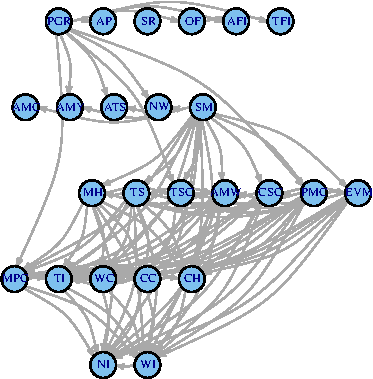
\includegraphics{pDag_dairy_cattle_data_files/figure-latex/network5-1.pdf}

\begin{Shaded}
\begin{Highlighting}[]
\NormalTok{B =}\StringTok{ }\KeywordTok{pcalg_custom}\NormalTok{(}\DataTypeTok{X =} \KeywordTok{as.matrix}\NormalTok{(data),}
                 \DataTypeTok{a =} \FloatTok{0.99}\NormalTok{)}\OperatorTok{$}\NormalTok{B}
\KeywordTok{colnames}\NormalTok{(B) =}\StringTok{ }\KeywordTok{colnames}\NormalTok{(data)}
\KeywordTok{row.names}\NormalTok{(B) =}\StringTok{ }\KeywordTok{colnames}\NormalTok{(data)}
\NormalTok{B =}\StringTok{ }\NormalTok{B[}\KeywordTok{invPerm}\NormalTok{(rand_ordr),}\KeywordTok{invPerm}\NormalTok{(rand_ordr)]}
\NormalTok{graphB =}\StringTok{ }\KeywordTok{graph_from_adjacency_matrix}\NormalTok{(}\KeywordTok{t}\NormalTok{(B), }\DataTypeTok{mode =} \StringTok{'directed'}\NormalTok{, }\DataTypeTok{weighted =} \OtherTok{TRUE}\NormalTok{, }\DataTypeTok{diag =} \OtherTok{FALSE}\NormalTok{)}
\KeywordTok{plot}\NormalTok{(graphB, }\DataTypeTok{layout =} \KeywordTok{coords5wTI}\NormalTok{(), }\DataTypeTok{vertex.size=}\DecValTok{15}\NormalTok{, }\DataTypeTok{vertex.label.dist =} \FloatTok{.1}\NormalTok{, }\DataTypeTok{vertex.color =} \StringTok{'SkyBlue2'}\NormalTok{,}
     \DataTypeTok{vertex.label.cex =} \FloatTok{0.5}\NormalTok{, }\DataTypeTok{edge.arrow.size =} \FloatTok{0.25}\NormalTok{, }\DataTypeTok{edge.curved=}\NormalTok{.}\DecValTok{3}\NormalTok{)}
\end{Highlighting}
\end{Shaded}

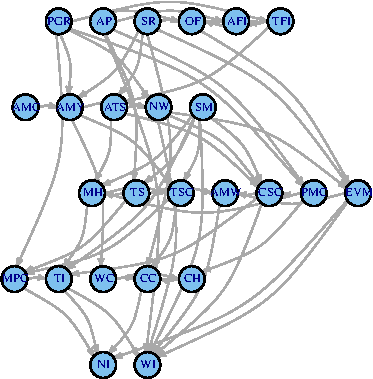
\includegraphics{pDag_dairy_cattle_data_files/figure-latex/network5pdag-1.pdf}

\begin{Shaded}
\begin{Highlighting}[]
\NormalTok{B =}\StringTok{ }\KeywordTok{pcalg_addBG5_t}\NormalTok{(}\DataTypeTok{X =} \KeywordTok{as.matrix}\NormalTok{(data),}
                 \DataTypeTok{a =} \FloatTok{0.99}\NormalTok{,}
                 \DataTypeTok{m1 =} \DecValTok{6}\NormalTok{, }
                 \DataTypeTok{m2 =} \DecValTok{11}\NormalTok{, }
                 \DataTypeTok{m3 =} \DecValTok{18}\NormalTok{, }
                 \DataTypeTok{m4 =} \DecValTok{23}\NormalTok{)}\OperatorTok{$}\NormalTok{B}
\KeywordTok{colnames}\NormalTok{(B) =}\StringTok{ }\KeywordTok{colnames}\NormalTok{(data)}
\KeywordTok{row.names}\NormalTok{(B) =}\StringTok{ }\KeywordTok{colnames}\NormalTok{(data)}
\NormalTok{B =}\StringTok{ }\NormalTok{B[}\KeywordTok{invPerm}\NormalTok{(rand_ordr),}\KeywordTok{invPerm}\NormalTok{(rand_ordr)]}
\NormalTok{graphB =}\StringTok{ }\KeywordTok{graph_from_adjacency_matrix}\NormalTok{(}\KeywordTok{t}\NormalTok{(B), }\DataTypeTok{mode =} \StringTok{'directed'}\NormalTok{, }\DataTypeTok{weighted =} \OtherTok{TRUE}\NormalTok{, }\DataTypeTok{diag =} \OtherTok{FALSE}\NormalTok{)}
\KeywordTok{plot}\NormalTok{(graphB, }\DataTypeTok{layout =} \KeywordTok{coords5wTI}\NormalTok{(), }\DataTypeTok{vertex.size=}\DecValTok{15}\NormalTok{, }\DataTypeTok{vertex.label.dist =} \FloatTok{.1}\NormalTok{, }\DataTypeTok{vertex.color =} \StringTok{'SkyBlue2'}\NormalTok{,}
     \DataTypeTok{vertex.label.cex =} \FloatTok{0.5}\NormalTok{, }\DataTypeTok{edge.arrow.size =} \FloatTok{0.25}\NormalTok{, }\DataTypeTok{edge.curved=}\NormalTok{.}\DecValTok{3}\NormalTok{)}
\end{Highlighting}
\end{Shaded}

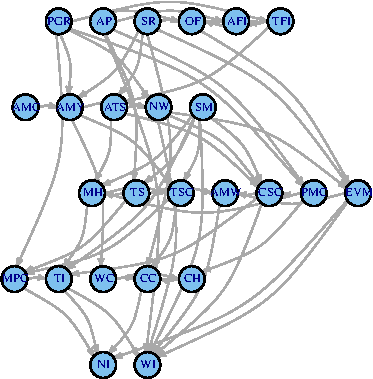
\includegraphics{pDag_dairy_cattle_data_files/figure-latex/network5pdagBGt-1.pdf}

\begin{Shaded}
\begin{Highlighting}[]
\NormalTok{B =}\StringTok{ }\KeywordTok{pcalg_addBG5}\NormalTok{(}\DataTypeTok{X =} \KeywordTok{as.matrix}\NormalTok{(data),}
                 \DataTypeTok{a =} \FloatTok{0.99}\NormalTok{,}
                 \DataTypeTok{m1 =} \DecValTok{6}\NormalTok{, }
                 \DataTypeTok{m2 =} \DecValTok{11}\NormalTok{, }
                 \DataTypeTok{m3 =} \DecValTok{18}\NormalTok{, }
                 \DataTypeTok{m4 =} \DecValTok{23}\NormalTok{)}\OperatorTok{$}\NormalTok{B}
\KeywordTok{colnames}\NormalTok{(B) =}\StringTok{ }\KeywordTok{colnames}\NormalTok{(data)}
\KeywordTok{row.names}\NormalTok{(B) =}\StringTok{ }\KeywordTok{colnames}\NormalTok{(data)}
\NormalTok{B =}\StringTok{ }\NormalTok{B[}\KeywordTok{invPerm}\NormalTok{(rand_ordr),}\KeywordTok{invPerm}\NormalTok{(rand_ordr)]}
\NormalTok{graphB =}\StringTok{ }\KeywordTok{graph_from_adjacency_matrix}\NormalTok{(}\KeywordTok{t}\NormalTok{(B), }\DataTypeTok{mode =} \StringTok{'directed'}\NormalTok{, }\DataTypeTok{weighted =} \OtherTok{TRUE}\NormalTok{, }\DataTypeTok{diag =} \OtherTok{FALSE}\NormalTok{)}
\KeywordTok{plot}\NormalTok{(graphB, }\DataTypeTok{layout =} \KeywordTok{coords5wTI}\NormalTok{(), }\DataTypeTok{vertex.size=}\DecValTok{15}\NormalTok{, }\DataTypeTok{vertex.label.dist =} \FloatTok{.1}\NormalTok{, }\DataTypeTok{vertex.color =} \StringTok{'SkyBlue2'}\NormalTok{,}
     \DataTypeTok{vertex.label.cex =} \FloatTok{0.5}\NormalTok{, }\DataTypeTok{edge.arrow.size =} \FloatTok{0.25}\NormalTok{, }\DataTypeTok{edge.curved=}\NormalTok{.}\DecValTok{3}\NormalTok{)}
\end{Highlighting}
\end{Shaded}

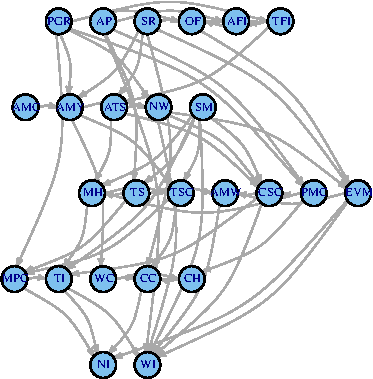
\includegraphics{pDag_dairy_cattle_data_files/figure-latex/network5pdagBG-1.pdf}

\hypertarget{group-network-1}{%
\subsubsection{10 group network}\label{group-network-1}}

In this section we run partition Dag with 10 groups:

\begin{Shaded}
\begin{Highlighting}[]
\NormalTok{lambda =}\StringTok{ }\DecValTok{4}
\NormalTok{B =}\StringTok{ }\NormalTok{partitionDAG}\OperatorTok{::}\KeywordTok{partial9}\NormalTok{(}\DataTypeTok{X =} \KeywordTok{as.matrix}\NormalTok{(data),}
                            \DataTypeTok{l =}\NormalTok{ lambda, }
                            \DataTypeTok{m1 =} \DecValTok{2}\NormalTok{, }
                            \DataTypeTok{m2 =} \DecValTok{3}\NormalTok{, }
                            \DataTypeTok{m3 =} \DecValTok{4}\NormalTok{, }
                            \DataTypeTok{m4 =} \DecValTok{6}\NormalTok{, }
                            \DataTypeTok{m5 =} \DecValTok{9}\NormalTok{,}
                            \DataTypeTok{m6 =} \DecValTok{11}\NormalTok{, }
                            \DataTypeTok{m7 =} \DecValTok{18}\NormalTok{, }
                            \DataTypeTok{m8 =} \DecValTok{23}\NormalTok{)}\OperatorTok{$}\NormalTok{B}
\KeywordTok{colnames}\NormalTok{(B) =}\StringTok{ }\KeywordTok{colnames}\NormalTok{(data)}
\KeywordTok{row.names}\NormalTok{(B) =}\StringTok{ }\KeywordTok{colnames}\NormalTok{(data)}
\NormalTok{B =}\StringTok{ }\NormalTok{B[}\KeywordTok{invPerm}\NormalTok{(rand_ordr),}\KeywordTok{invPerm}\NormalTok{(rand_ordr)]}
\NormalTok{graphB =}\StringTok{ }\KeywordTok{graph_from_adjacency_matrix}\NormalTok{(}\KeywordTok{t}\NormalTok{(B), }\DataTypeTok{mode =} \StringTok{'directed'}\NormalTok{, }\DataTypeTok{weighted =} \OtherTok{TRUE}\NormalTok{, }\DataTypeTok{diag =} \OtherTok{FALSE}\NormalTok{)}
\KeywordTok{plot}\NormalTok{(graphB, }\DataTypeTok{layout =} \KeywordTok{coords9wTI}\NormalTok{(), }\DataTypeTok{vertex.size=}\DecValTok{15}\NormalTok{, }\DataTypeTok{vertex.label.dist =} \FloatTok{.1}\NormalTok{, }\DataTypeTok{vertex.color =} \StringTok{'SkyBlue2'}\NormalTok{,}
     \DataTypeTok{vertex.label.cex =} \FloatTok{0.5}\NormalTok{, }\DataTypeTok{edge.arrow.size =} \FloatTok{0.25}\NormalTok{, }\DataTypeTok{edge.curved=}\NormalTok{.}\DecValTok{3}\NormalTok{)}
\end{Highlighting}
\end{Shaded}

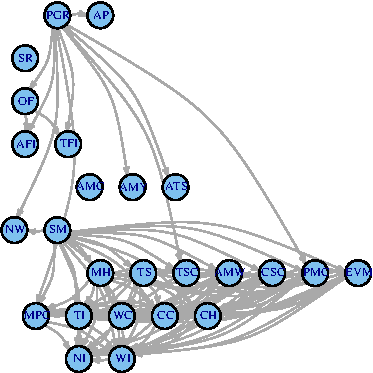
\includegraphics{pDag_dairy_cattle_data_files/figure-latex/network10-1.pdf}

\end{document}
